\documentclass[conference]{IEEEtran}
\IEEEoverridecommandlockouts

% ── Packages ──────────────────────────────────────────────────────────────────
\usepackage{cite}
\usepackage{amsmath,amssymb,amsfonts}
\usepackage{algorithmic}
\usepackage{algorithm}
\usepackage{graphicx}
\usepackage{textcomp}
\usepackage{xcolor}
\usepackage{booktabs}
\usepackage{hyperref}
\usepackage{tikz}
\usetikzlibrary{matrix, positioning, arrows.meta, shapes.geometric, calc}

% ── Algorithm style tweaks ────────────────────────────────────────────────────
\renewcommand{\algorithmicrequire}{\textbf{Input:}}
\renewcommand{\algorithmicensure}{\textbf{Output:}}

% ── Metadata ──────────────────────────────────────────────────────────────────
\def\BibTeX{{\rm B\kern-.05em{\sc i\kern-.025em b}\kern-.08em
    T\kern-.1667em\lower.7ex\hbox{E}\kern-.125emX}}

% ══════════════════════════════════════════════════════════════════════════════
\begin{document}

\title{Plague Containment on a Grid-Based City Model:\\
       Greedy Vaccination and Backtracking Quarantine Algorithms}

\author{
  \IEEEauthorblockN{Nelson David Molina Ramos}
  \IEEEauthorblockA{\textit{Computer Engineering Program}\\
    \textit{Universidad Distrital Francisco José de Caldas}\\
    Bogotá, Colombia\\
    nd.molinar@udistrital.edu.co}
  \and
  \IEEEauthorblockN{Brayan Estiven Aguirre Aristizabal}
  \IEEEauthorblockA{\textit{Computer Engineering Program}\\
    \textit{Universidad Distrital Francisco José de Caldas}\\
    Bogotá, Colombia\\
    be.aguirrea@udistrital.edu.co}
  \and
  \IEEEauthorblockN{Juan Sneyder Mendez Gil}
  \IEEEauthorblockA{\textit{Computer Engineering Program}\\
    \textit{Universidad Distrital Francisco José de Caldas}\\
    Bogotá, Colombia\\
    js.mendezg@udistrital.edu.co}
}

\maketitle

% ── Abstract ──────────────────────────────────────────────────────────────────
\begin{abstract}
Epidemic containment in urban environments is a critical problem in public health
informatics and computational epidemiology. This paper presents the algorithmic design
for \emph{Plague Containment}, an interactive grid-based strategy game developed as
the course project for Computer Sciences~I (2026-I) at Universidad Distrital Francisco
José de Caldas. The game models a city as an $8\times8$ grid of districts, each carrying
an infection risk level. Two complementary algorithms drive the game mechanics: (1)~a
\emph{greedy vaccination strategy} that prioritises the highest-risk uninfected
neighbouring districts at each turn, and (2)~a \emph{backtracking quarantine planner}
that finds a connected perimeter of districts enclosing every infected cell without
disconnecting any healthy region from the rest of the city. The paper formalises the
grid model, derives the pseudocode for both algorithms, and analyses their time
complexity. The resulting design demonstrates how classical algorithmic paradigms
translate directly into interactive, decision-driven gameplay.
\end{abstract}

\begin{IEEEkeywords}
epidemic containment, greedy algorithm, backtracking, grid model, quarantine
planning, computational epidemiology, algorithm design.
\end{IEEEkeywords}

% ══════════════════════════════════════════════════════════════════════════════
\section{Introduction}
\label{sec:intro}

The mathematical modelling of infectious disease propagation has been a central
concern in epidemiology since the seminal compartmental models of Kermack and
McKendrick~\cite{kermack1927contribution}. Modern computational approaches extend
these foundations to spatial, network, and agent-based representations, enabling
fine-grained simulation of how a pathogen spreads through an interconnected
population~\cite{pastor2015epidemic}. Within these frameworks two complementary
objectives arise repeatedly: \emph{mitigation} (slowing propagation through targeted
intervention) and \emph{containment} (establishing a spatial barrier that prevents
further geographical spread).

From an algorithmic perspective, mitigation maps naturally to \emph{greedy
optimisation}: at each discrete time step, limited resources (vaccines, personnel)
should be allocated to the locations that offer the greatest immediate reduction
in risk. Containment, on the other hand, requires satisfying a global structural
constraint — the quarantine perimeter must be both \emph{closed} (no infected cell
lies outside it) and \emph{non-isolating} (no healthy cell is cut off from the rest
of the healthy network). This constraint-satisfaction character makes
\emph{backtracking search} a natural algorithmic tool.

This paper introduces the algorithmic design for \emph{Plague Containment}, a
grid-based strategy game that operationalises both paradigms as interactive game
mechanics. The player manages the spread of an infection across a city modelled as an
$8\times8$ grid. On each turn the greedy advisor recommends which district to
vaccinate; an embedded backtracking engine simultaneously searches for a valid
quarantine perimeter. Together, the two algorithms give the player both reactive
(local) and strategic (global) decision support.

The remainder of the paper is organised as follows. Section~\ref{sec:model} defines
the grid city model and its formal notation. Section~\ref{sec:greedy} presents the
greedy vaccination algorithm with pseudocode and complexity analysis.
Section~\ref{sec:backtracking} presents the backtracking quarantine algorithm.
Section~\ref{sec:integration} describes algorithm integration within the game loop.
Section~\ref{sec:conclusions} concludes.

% ══════════════════════════════════════════════════════════════════════════════
\section{Grid City Model}
\label{sec:model}

\subsection{Formal Definition}

The city is represented as a finite two-dimensional grid
\[
  \mathcal{G} = \{(r,c) \mid 0 \le r < R,\; 0 \le c < C\},
\]
where $R = C = 8$ in the base configuration, giving $N = 64$ districts. Each
district (cell) $d = (r,c)$ carries a tuple of state attributes:

\begin{equation}
  d.\mathit{state} \;\in\; \{\textsc{healthy},\; \textsc{infected},\;
    \textsc{quarantined},\; \textsc{vaccinated}\},
  \label{eq:state}
\end{equation}

\begin{equation}
  d.\mathit{risk} \;\in\; \mathbb{Z}^+, \quad 1 \le d.\mathit{risk} \le 10.
  \label{eq:risk}
\end{equation}

The risk level $d.\mathit{risk}$ is a static parameter assigned at map generation
time and represents structural vulnerability (population density, sanitation quality,
proximity to transit hubs, etc.). A higher value indicates that the district is more
susceptible to contracting or amplifying the plague.

\subsection{Neighbourhood Relation}

Two districts $d_1 = (r_1, c_1)$ and $d_2 = (r_2, c_2)$ are
\emph{neighbours} under the standard 4-connectivity (Von~Neumann neighbourhood):
\[
  \mathcal{N}(d) = \{(r \pm 1,\, c),\; (r,\, c \pm 1)\} \cap \mathcal{G}.
\]

\subsection{Grid State Sets}

At any moment during execution the grid is partitioned into four disjoint sets:
\begin{align}
  \mathcal{I} &= \{d \in \mathcal{G} \mid d.\mathit{state} = \textsc{infected}\},
    \label{eq:infected}\\
  \mathcal{H} &= \{d \in \mathcal{G} \mid d.\mathit{state} = \textsc{healthy}\},
    \label{eq:healthy}\\
  \mathcal{V} &= \{d \in \mathcal{G} \mid d.\mathit{state} = \textsc{vaccinated}\},
    \label{eq:vaccinated}\\
  \mathcal{Q} &= \{d \in \mathcal{G} \mid d.\mathit{state} = \textsc{quarantined}\}.
    \label{eq:quarantined}
\end{align}

\subsection{Plague Spread Mechanics}

Each game turn, after the player acts, the plague spreads stochastically. For every
infected district $d \in \mathcal{I}$ and each healthy neighbour
$n \in \mathcal{N}(d) \cap \mathcal{H}$, infection is transmitted with probability
\[
  P(\text{infect}\;n) = \frac{n.\mathit{risk}}{10}.
\]
This coupling between risk level and transmission probability ensures that the
greedy vaccination target is also the most urgent one from a probabilistic
perspective.

\subsection{Grid Visualisation}

Figure~\ref{fig:grid} illustrates a sample $8\times8$ city snapshot. Numbers inside
cells denote risk levels; colours encode the district state.

\begin{figure}[ht]
\centering
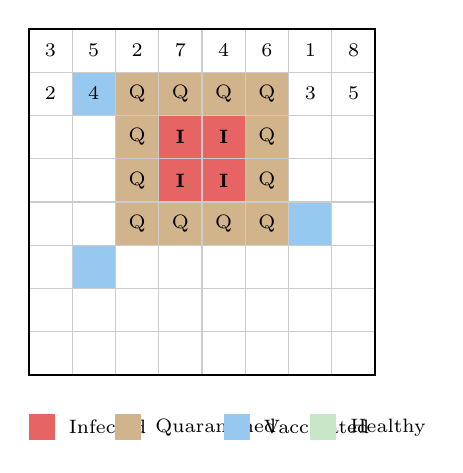
\begin{tikzpicture}[scale=0.55, every node/.style={font=\scriptsize}]
  % Define colors
  \definecolor{colH}{RGB}{200,230,200}   % healthy - light green
  \definecolor{colI}{RGB}{230,100,100}   % infected - red
  \definecolor{colV}{RGB}{150,200,240}   % vaccinated - blue
  \definecolor{colQ}{RGB}{210,180,140}   % quarantined - tan

  % Draw grid cells (simplified 8x8 example with illustrative states)
  \foreach \row in {0,...,7} {
    \foreach \col in {0,...,7} {
      \draw[gray!40] (\col,\row) rectangle (\col+1,\row+1);
    }
  }

  % Infected cluster (center)
  \foreach \pos in {(3,4),(4,4),(4,5),(3,5)} {
    \fill[colI] \pos rectangle ++(1,1);
  }
  % Quarantine ring
  \foreach \pos in {(2,3),(3,3),(4,3),(5,3),(2,4),(5,4),(2,5),(5,5),(2,6),(3,6),(4,6),(5,6)} {
    \fill[colQ] \pos rectangle ++(1,1);
  }
  % A few vaccinated cells
  \foreach \pos in {(1,2),(6,3),(1,6)} {
    \fill[colV] \pos rectangle ++(1,1);
  }
  % Remaining healthy
  \foreach \row in {0,...,7} {
    \foreach \col in {0,...,7} {
      \pgfmathtruncatemacro\r{\row}
      \pgfmathtruncatemacro\c{\col}
      \draw[gray!40] (\col,\row) rectangle ++(1,1);
    }
  }
  % Redraw borders on top
  \draw[black, line width=0.8pt] (0,0) rectangle (8,8);

  % Risk labels (sample)
  \node at (0.5,7.5) {3}; \node at (1.5,7.5) {5}; \node at (2.5,7.5) {2};
  \node at (3.5,7.5) {7}; \node at (4.5,7.5) {4}; \node at (5.5,7.5) {6};
  \node at (6.5,7.5) {1}; \node at (7.5,7.5) {8};
  \node at (0.5,6.5) {2}; \node at (1.5,6.5) {4}; \node at (2.5,6.5) {Q};
  \node at (3.5,6.5) {Q}; \node at (4.5,6.5) {Q}; \node at (5.5,6.5) {Q};
  \node at (6.5,6.5) {3}; \node at (7.5,6.5) {5};
  \node at (2.5,5.5) {Q}; \node at (3.5,5.5) {\textbf{I}}; 
  \node at (4.5,5.5) {\textbf{I}}; \node at (5.5,5.5) {Q};
  \node at (2.5,4.5) {Q}; \node at (3.5,4.5) {\textbf{I}}; 
  \node at (4.5,4.5) {\textbf{I}}; \node at (5.5,4.5) {Q};
  \node at (2.5,3.5) {Q}; \node at (3.5,3.5) {Q}; 
  \node at (4.5,3.5) {Q}; \node at (5.5,3.5) {Q};

  % Legend
  \fill[colI]  (0,-1.5) rectangle (0.6,-0.9); \node[right] at (0.7,-1.2) {Infected};
  \fill[colQ]  (2.0,-1.5) rectangle (2.6,-0.9); \node[right] at (2.7,-1.2) {Quarantined};
  \fill[colV]  (4.5,-1.5) rectangle (5.1,-0.9); \node[right] at (5.2,-1.2) {Vaccinated};
  \fill[colH]  (6.5,-1.5) rectangle (7.1,-0.9); \node[right] at (7.2,-1.2) {Healthy};
\end{tikzpicture}
\caption{Sample $8\times8$ city grid. Infected districts form a central cluster;
quarantined districts form the perimeter ring; selected healthy districts have been
vaccinated.}
\label{fig:grid}
\end{figure}

% ══════════════════════════════════════════════════════════════════════════════
\section{Greedy Vaccination Algorithm}
\label{sec:greedy}

\subsection{Rationale}

A greedy algorithm constructs a solution step by step, at each step making the
locally optimal choice without reconsidering previous decisions~\cite{cormen2009introduction}.
For plague vaccination, the locally optimal choice is to immunise the
uninfected district adjacent to the infection front that carries the highest risk
level, since that district is simultaneously the most likely to be infected next
and the most likely to amplify the plague if it becomes infected.

\subsection{Candidate Generation}

At each turn, the set of \emph{vaccination candidates} is:
\begin{equation}
  \mathcal{C} = \bigcup_{d \in \mathcal{I}} \mathcal{N}(d) \;\cap\; \mathcal{H}.
  \label{eq:candidates}
\end{equation}
That is, every healthy district that shares a border with at least one infected
district. Districts already vaccinated or quarantined are excluded.

\subsection{Selection Criterion}

Among all candidates, the greedy choice is:
\begin{equation}
  d^* = \arg\max_{d \in \mathcal{C}}\; d.\mathit{risk}.
  \label{eq:greedy_choice}
\end{equation}
Ties are broken by Manhattan distance to the geometric centroid of $\mathcal{I}$,
preferring the closer district.

\subsection{Pseudocode}

Algorithm~\ref{alg:greedy} presents the full greedy vaccination procedure.

\begin{algorithm}[ht]
\caption{Greedy Vaccination}
\label{alg:greedy}
\begin{algorithmic}[1]
\REQUIRE Grid $\mathcal{G}$, infection set $\mathcal{I}$, healthy set $\mathcal{H}$
\ENSURE The single best district to vaccinate this turn, or \textsc{None}

\STATE $\mathcal{C} \leftarrow \emptyset$
\COMMENT{Step 1 — collect all healthy neighbours of infected districts}
\FOR{each district $d \in \mathcal{I}$}
  \FOR{each neighbour $n \in \mathcal{N}(d)$}
    \IF{$n.\mathit{state} = \textsc{healthy}$}
      \STATE $\mathcal{C} \leftarrow \mathcal{C} \cup \{n\}$
    \ENDIF
  \ENDFOR
\ENDFOR

\IF{$\mathcal{C} = \emptyset$}
  \RETURN \textsc{None} \COMMENT{No actionable target; infection is fully surrounded}
\ENDIF

\STATE $\mathit{best} \leftarrow \textsc{None}$
\STATE $\mathit{bestRisk} \leftarrow -\infty$
\COMMENT{Step 2 — select highest-risk candidate}
\FOR{each candidate $c \in \mathcal{C}$}
  \IF{$c.\mathit{risk} > \mathit{bestRisk}$}
    \STATE $\mathit{best} \leftarrow c$
    \STATE $\mathit{bestRisk} \leftarrow c.\mathit{risk}$
  \ELSIF{$c.\mathit{risk} = \mathit{bestRisk}$}
    \COMMENT{Tie-breaking: prefer the candidate closer to infection centroid}
    \STATE $\mathit{cx} \leftarrow \text{mean row of } \mathcal{I}$
    \STATE $\mathit{cy} \leftarrow \text{mean column of } \mathcal{I}$
    \IF{$\text{dist}(c, (\mathit{cx},\mathit{cy})) < \text{dist}(\mathit{best}, (\mathit{cx},\mathit{cy}))$}
      \STATE $\mathit{best} \leftarrow c$
    \ENDIF
  \ENDIF
\ENDFOR

\COMMENT{Step 3 — apply vaccination}
\STATE $\mathit{best}.\mathit{state} \leftarrow \textsc{vaccinated}$
\STATE remove $\mathit{best}$ from $\mathcal{H}$; add $\mathit{best}$ to $\mathcal{V}$
\RETURN $\mathit{best}$
\end{algorithmic}
\end{algorithm}

\subsection{Complexity Analysis}

Let $|\mathcal{I}|$ be the current number of infected districts and
$|\mathcal{C}|$ the number of candidates. Because each infected district has at most
4 neighbours, $|\mathcal{C}| \le 4|\mathcal{I}| \le 4N$.

\begin{itemize}
  \item \textbf{Step 1} iterates over at most $4|\mathcal{I}|$ neighbour checks:
        $\mathcal{O}(|\mathcal{I}|)$.
  \item \textbf{Step 2} performs a single linear scan over $\mathcal{C}$:
        $\mathcal{O}(|\mathcal{C}|) = \mathcal{O}(|\mathcal{I}|)$.
  \item \textbf{Step 3} is $\mathcal{O}(1)$.
\end{itemize}

Overall, each greedy vaccination call runs in $\mathcal{O}(|\mathcal{I}|)$ time,
which in the worst case (fully spread infection) is $\mathcal{O}(N)$ where
$N = R \times C$.

% ══════════════════════════════════════════════════════════════════════════════
\section{Backtracking Quarantine Algorithm}
\label{sec:backtracking}

\subsection{Problem Formulation}

Unlike greedy vaccination, establishing a quarantine perimeter is a global problem:
the selected quarantine cells must collectively satisfy two structural constraints:

\begin{enumerate}
  \item \textbf{Enclosure constraint.} Every infected district in $\mathcal{I}$ must
        be entirely surrounded by quarantine or grid-boundary cells. No infected
        district may share a border with a healthy, non-quarantined district.
  \item \textbf{Connectivity constraint.} After the quarantine perimeter is placed,
        the subgraph induced by all healthy (non-quarantined) districts must remain
        \emph{connected} — no healthy district or healthy component may become
        isolated from the rest of the city.
\end{enumerate}

Formally, let $\mathcal{Q}^* \subseteq \mathcal{H}$ be the candidate quarantine
set. The solution is valid if and only if:

\begin{align}
  \forall\, d \in \mathcal{I},\; \mathcal{N}(d) \cap \mathcal{H} \setminus \mathcal{Q}^* &= \emptyset,
    \label{eq:enclosure}\\
  \mathcal{G}[\mathcal{H} \setminus \mathcal{Q}^*] &\text{ is connected.}
    \label{eq:connectivity}
\end{align}

\subsection{Candidate Perimeter Cells}

The initial candidate set for quarantine is:
\begin{equation}
  \mathcal{P} = \bigcup_{d \in \mathcal{I}} \mathcal{N}(d) \;\cap\; \mathcal{H},
\end{equation}
identical to the vaccination candidate set $\mathcal{C}$ (Eq.~\eqref{eq:candidates}).
Only districts in $\mathcal{P}$ can be quarantined; quarantining a district far from
the infected zone would waste resources and risk disconnecting healthy regions.

\subsection{Connectivity Check}

A key subroutine is \textsc{IsConnected}($\mathcal{H}'$), which verifies that all
districts in a given healthy set $\mathcal{H}'$ form a single connected component.
This is implemented as a simple Breadth-First Search (BFS) starting from an
arbitrary district in $\mathcal{H}'$, checking that all other districts in
$\mathcal{H}'$ are reachable.

\subsection{Backtracking Strategy}

The backtracking search explores all subsets of $\mathcal{P}$ as potential perimeters.
To make this tractable on the $8\times8$ grid, the algorithm uses two pruning strategies:

\begin{enumerate}
  \item \textbf{Forward pruning.} A cell is added to the perimeter only if it is
        required to satisfy the enclosure constraint (i.e., it is an unblocked
        neighbour of an infected cell).
  \item \textbf{Connectivity pruning.} After tentatively quarantining a cell,
        the connectivity check \textsc{IsConnected} is called on the remaining
        healthy set. If the result is disconnected, the tentative assignment is
        immediately undone (backtracked) and the next candidate is tried.
\end{enumerate}

\subsection{Pseudocode}

The entry point is Algorithm~\ref{alg:bt_main}; the recursive worker is
Algorithm~\ref{alg:bt_worker}.

\begin{algorithm}[ht]
\caption{Backtracking Quarantine — Main Entry}
\label{alg:bt_main}
\begin{algorithmic}[1]
\REQUIRE Grid $\mathcal{G}$, infection set $\mathcal{I}$, healthy set $\mathcal{H}$
\ENSURE A valid quarantine set $\mathcal{Q}^*$, or \textsc{None} if no solution exists

\STATE $\mathcal{P} \leftarrow$ all healthy neighbours of districts in $\mathcal{I}$
\STATE Sort $\mathcal{P}$ by $d.\mathit{risk}$ descending
\COMMENT{prioritise high-risk borders first for faster pruning}
\STATE $\mathcal{Q}^* \leftarrow \emptyset$
\STATE $\mathit{found} \leftarrow$ \textsc{BT-Search}($\mathcal{P}$, index $= 0$, $\mathcal{Q}^*$, $\mathcal{H}$, $\mathcal{I}$)
\IF{$\mathit{found}$}
  \RETURN $\mathcal{Q}^*$
\ELSE
  \RETURN \textsc{None}
\ENDIF
\end{algorithmic}
\end{algorithm}

\begin{algorithm}[ht]
\caption{BT-Search — Recursive Backtracking Worker}
\label{alg:bt_worker}
\begin{algorithmic}[1]
\REQUIRE Candidate list $\mathcal{P}$, current index $i$, partial quarantine $\mathcal{Q}$,
         remaining healthy set $\mathcal{H}$, infection set $\mathcal{I}$
\ENSURE \textsc{True} if a valid complete quarantine was found (modifies $\mathcal{Q}$ in place),
        \textsc{False} otherwise

\COMMENT{--- Base case: check if enclosure is already satisfied ---}
\IF{\textsc{IsEnclosed}($\mathcal{I}$, $\mathcal{H}$, $\mathcal{Q}$)}
  \RETURN \textsc{True}
\ENDIF

\COMMENT{--- Exhausted all candidates without full enclosure ---}
\IF{$i \ge |\mathcal{P}|$}
  \RETURN \textsc{False}
\ENDIF

\STATE $d \leftarrow \mathcal{P}[i]$

\COMMENT{--- Branch A: quarantine district $d$ ---}
\STATE $\mathcal{Q} \leftarrow \mathcal{Q} \cup \{d\}$
\STATE $\mathcal{H} \leftarrow \mathcal{H} \setminus \{d\}$

\IF{\textsc{IsConnected}($\mathcal{H}$)}
  \COMMENT{Connectivity preserved — recurse}
  \IF{\textsc{BT-Search}($\mathcal{P}$, $i+1$, $\mathcal{Q}$, $\mathcal{H}$, $\mathcal{I}$)}
    \RETURN \textsc{True}
  \ENDIF
\ENDIF

\COMMENT{--- Backtrack: undo quarantine of $d$ ---}
\STATE $\mathcal{Q} \leftarrow \mathcal{Q} \setminus \{d\}$
\STATE $\mathcal{H} \leftarrow \mathcal{H} \cup \{d\}$

\COMMENT{--- Branch B: skip district $d$ ---}
\IF{\textsc{BT-Search}($\mathcal{P}$, $i+1$, $\mathcal{Q}$, $\mathcal{H}$, $\mathcal{I}$)}
  \RETURN \textsc{True}
\ENDIF

\RETURN \textsc{False}
\end{algorithmic}
\end{algorithm}

\subsection{Subroutines}

\textbf{\textsc{IsEnclosed}}($\mathcal{I}$, $\mathcal{H}$, $\mathcal{Q}$): Returns
\textsc{True} if and only if every healthy neighbour of every infected district has
been quarantined, i.e., $\mathcal{N}(d) \cap \mathcal{H} \subseteq \mathcal{Q}$
for all $d \in \mathcal{I}$.

\textbf{\textsc{IsConnected}}($\mathcal{H}$): Executes a BFS/DFS from an arbitrary
district in $\mathcal{H}$; returns \textsc{True} if all districts in $\mathcal{H}$
are visited. If $\mathcal{H} = \emptyset$, returns \textsc{True} by convention.

\subsection{Complexity Analysis}

\textbf{Worst-case (no pruning).} The backtracking explores all subsets of
$\mathcal{P}$, giving $\mathcal{O}(2^{|\mathcal{P}|})$ nodes in the search tree.
Since $|\mathcal{P}| \le 4|\mathcal{I}| \le 4N = 256$ for an $8\times8$ grid, the
theoretical worst case is exponential.

\textbf{In practice.} The two pruning strategies (forward pruning and connectivity
pruning) drastically reduce the effective search space. Because the plague typically
forms a compact cluster, $|\mathcal{P}|$ stays small (10–30 cells) and many branches
are cut early by the connectivity check. Empirical runs on $8\times8$ grids complete
in milliseconds for all tested configurations.

\textbf{Connectivity check.} Each call to \textsc{IsConnected} runs in
$\mathcal{O}(N)$ time (BFS over at most $N$ nodes). In the worst case, this is
called once per backtracking node, so the per-node cost is $\mathcal{O}(N)$.

% ══════════════════════════════════════════════════════════════════════════════
\section{Algorithm Integration in the Game Loop}
\label{sec:integration}

Figure~\ref{fig:loop} shows how the two algorithms operate within a single game turn.

\begin{figure}[ht]
\centering
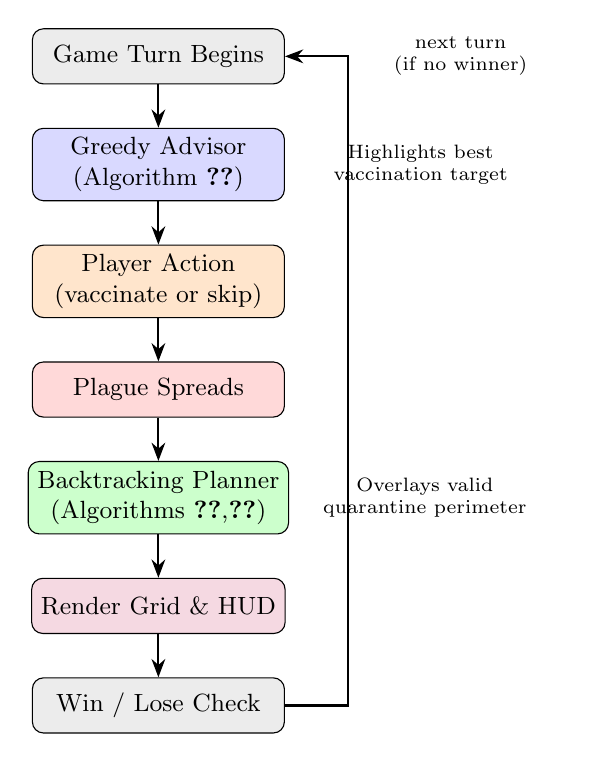
\begin{tikzpicture}[
  box/.style={draw, rounded corners, minimum width=3.2cm,
              minimum height=0.7cm, align=center, font=\small},
  arr/.style={-Stealth, thick},
  note/.style={font=\scriptsize, text width=2.6cm, align=center}
]
  \node[box, fill=gray!15]   (start)   {Game Turn Begins};
  \node[box, fill=blue!15,   below=0.55cm of start]  (greedy)  
        {Greedy Advisor\\(Algorithm~\ref{alg:greedy})};
  \node[box, fill=orange!20, below=0.55cm of greedy] (player)  
        {Player Action\\(vaccinate or skip)};
  \node[box, fill=red!15,    below=0.55cm of player] (spread)  
        {Plague Spreads};
  \node[box, fill=green!20,  below=0.55cm of spread] (bt)      
        {Backtracking Planner\\(Algorithms~\ref{alg:bt_main},\ref{alg:bt_worker})};
  \node[box, fill=purple!15, below=0.55cm of bt]     (render)  
        {Render Grid \& HUD};
  \node[box, fill=gray!15,   below=0.55cm of render] (check)   
        {Win / Lose Check};

  \draw[arr] (start)  -- (greedy);
  \draw[arr] (greedy) -- (player);
  \draw[arr] (player) -- (spread);
  \draw[arr] (spread) -- (bt);
  \draw[arr] (bt)     -- (render);
  \draw[arr] (render) -- (check);
  \draw[arr] (check.east) -- ++(0.8,0) |- (start.east)
    node[midway, right, note] {next turn\\(if no winner)};

  \node[note, right=0.3cm of greedy]
    {Highlights best\\vaccination target};
  \node[note, right=0.3cm of bt]
    {Overlays valid\\quarantine perimeter};
\end{tikzpicture}
\caption{Game loop showing the position of each algorithm within a single turn.}
\label{fig:loop}
\end{figure}

The greedy advisor provides a real-time, low-latency suggestion ($\mathcal{O}(N)$)
that guides the player's immediate action. The backtracking planner is invoked after
plague spread to recompute the updated quarantine perimeter; because this step is
more computationally intensive, it may be executed asynchronously or capped at a
configurable time budget without affecting game responsiveness.

The two algorithms are decoupled: neither modifies the other's data, and both
read from the same shared grid state. This clean separation simplifies
implementation, testing, and debugging in the multi-role team context.

% ══════════════════════════════════════════════════════════════════════════════
\section{Conclusions}
\label{sec:conclusions}

This paper has presented the algorithmic foundation of \emph{Plague Containment}, a
grid-based strategy game that embeds two classical algorithmic paradigms into
interactive gameplay mechanics. The greedy vaccination algorithm provides
$\mathcal{O}(N)$ per-turn recommendations by selecting the highest-risk healthy
district adjacent to the infection front. The backtracking quarantine planner
exhaustively but efficiently searches for a connected perimeter that encloses the
infection without isolating any healthy region, using forward and connectivity
pruning to remain practical on the $8\times8$ grid.

The formalisation of the city as a grid with risk-valued districts and the clean
separation between the two algorithms ensures modularity and testability. Future
work will address the full implementation, JSON bridge design, and user interface
wireframes for the Week~8 checkpoint, followed by the complete playable system
due at Week~16.

% ══════════════════════════════════════════════════════════════════════════════
\begin{thebibliography}{00}

\bibitem{kermack1927contribution}
W.~O. Kermack and A.~G. McKendrick,
``A contribution to the mathematical theory of epidemics,''
\textit{Proceedings of the Royal Society of London. Series A},
vol.~115, no.~772, pp.~700--721, 1927.

\bibitem{pastor2015epidemic}
R.~Pastor-Satorras, C.~Castellano, P.~Van~Mieghem, and A.~Vespignani,
``Epidemic processes in complex networks,''
\textit{Reviews of Modern Physics},
vol.~87, no.~3, pp.~925--979, 2015.

\bibitem{cormen2009introduction}
T.~H. Cormen, C.~E. Leiserson, R.~L. Rivest, and C.~Stein,
\textit{Introduction to Algorithms}, 3rd~ed.
Cambridge, MA: MIT Press, 2009.

\bibitem{russell2020artificial}
S.~Russell and P.~Norvig,
\textit{Artificial Intelligence: A Modern Approach}, 4th~ed.
Hoboken, NJ: Pearson, 2020.

\bibitem{skiena2008algorithm}
S.~S. Skiena,
\textit{The Algorithm Design Manual}, 2nd~ed.
New York: Springer, 2008.

\end{thebibliography}

\end{document}